\section{Langkah-Langkah Percobaan}
percobaan pertama yaitu melakukan crimping kabel LAN. Alat dan bahan yang digunakan adalah kabel LAN, konektor RJ45, crimping tool, dan tester. Langkah-langkah percobaan adalah sebagai berikut:
\begin{enumerate}
    \item Siapkan alat dan bahan yang diperlukan.
    \item Kupas ujung kabel LAN sekitar 1 ruas jari untuk mengeluarkan 8 kabel kecil di dalamnya.
    \item Urutkan kabel kecil sesuai dengan standar T568B.
    \item Luruskan kabel kecil dan potong ujungnya agar rata.
    \item Masukkan kabel kecil ke dalam konektor RJ45 hingga mentok di bagian dalam konektor.
    \item Gunakan crimping tool untuk menekan konektor RJ45 agar terpasang dengan baik pada kabel LAN.
    \item Ulangi langkah 2-6 untuk ujung kabel LAN yang satunya.
    \item Gunakan tester untuk memeriksa koneksi kabel LAN yang telah dibuat.
\end{enumerate}
percobaan kedua yaitu melakukan routing satis dan dinamis. namun, karena keterbatasan waktu dan ada beberapa kesalahan pada saat praktikum, praktikan hanya berhasil melakukan routing statis. Alat dan bahan yang digunakan adalah 2 buah router, 2 buah PC, dan 3 kabel LAN. Langkah-langkah percobaan routing statis adalah sebagai berikut:
\begin{enumerate}
    \item Siapkan alat dan bahan yang diperlukan.
    \item Matikan firewall pada masing-masing PC.
    \item Hubungkan kedua router dengan kabel LAN pada port WAN.
    \item Hubungkan masing-masing router dengan PC menggunakan kabel LAN pada port LAN.
    \item Buka app winbox pada masing-masing PC dan koneksikan ke router yang sesuai.
    \item Reset router ke kondisi awal atau default dengan masuk ke menu System > Reset Configuration.
    \item Konfigurasi IP address pada tiap interface router sesuai dengan topologi yang ditentukan dan dengan ip address yang ada pada modul praktikum dengan cara masuk ke menu IP > Addresses.
    \item Konfigurasi routing statis pada masing-masing router dengan cara masuk ke menu IP > Routes dengan Dst. Address sesuai dengan IP address yang ada pada modul praktikum dan Gateway sesuai dengan IP address router yang terhubung atau sesuai dengan pada modul praktikum.
    \item Konfigurasi IP address pada masing-masing PC sesuai dengan IP address yang ada pada modul praktikum dengan cara masuk ke Control Panel > Network and Sharing Center > Change adapter settings > klik kanan pada Local Area Connection > Properties > Internet Protocol Version 4 (TCP/IPv4) > Properties.
    \item Lakukan ping dari masing-masing PC ke router dan ke PC lainnya untuk memastikan koneksi berhasil.
    
\end{enumerate}
\section{Analisis Hasil Percobaan}Pada percobaan pertama yaitu crimping kabel LAN, praktikan berhasil melakukan proses penyusunan dan pemasangan konektor RJ45 pada kabel LAN menggunakan standar T568B. Hasil pengujian koneksi dengan menggunakan LAN tester menunjukkan bahwa semua pin terhubung dengan benar, yang berarti crimping berhasil dan kabel dapat digunakan untuk komunikasi data. Secara teori, jika urutan kabel sesuai standar dan crimping dilakukan dengan benar, maka kabel seharusnya dapat menghantarkan data dengan baik. Hasil percobaan ini sesuai dengan teori tersebut. Tidak terdapat kesalahan signifikan dalam tahap ini, karena alat yang digunakan berfungsi dengan baik dan langkah-langkah diikuti dengan cermat.

Faktor yang mendukung keberhasilan percobaan ini antara lain adalah penggunaan crimping tool yang masih dalam kondisi baik dan perhatian praktikan dalam memastikan urutan warna kabel sesuai standar. Namun, kesalahan yang bisa terjadi pada percobaan ini antara lain jika kabel tidak masuk sempurna ke konektor, atau crimping tidak dilakukan dengan tekanan yang cukup, yang dapat menyebabkan jalur data tidak tersambung.

Pada percobaan kedua yaitu routing jaringan, praktikan hanya berhasil melakukan routing statis karena keterbatasan waktu dan kendala teknis yang terjadi selama praktikum. Routing statis dilakukan dengan mengatur IP address pada masing-masing router dan PC, serta mengatur tabel routing secara manual pada masing-masing router. Hasil ping dari PC ke router dan antar PC menunjukkan bahwa koneksi berhasil terjalin, yang berarti konfigurasi routing statis telah dilakukan dengan benar. Hal ini sesuai dengan teori bahwa routing statis memungkinkan konektivitas antar jaringan jika alamat IP dan jalur (route) dikonfigurasi secara tepat.

Namun, tidak berhasilnya percobaan routing dinamis menunjukkan adanya hambatan dalam pelaksanaan praktikum, yang bisa disebabkan oleh beberapa faktor. Kemungkinan faktor yang memengaruhi antara lain adalah: Waktu praktikum yang terbatas sehingga konfigurasi routing dinamis tidak sempat dilakukan, terlalu lama dalam melakukan percobaan 1, dan kurangnya pemahaman awal terhadap langkah-langkah konfigurasi routing yang menyebabkan stuck pada saat praktikum.
Secara keseluruhan, praktikum ini berhasil dalam memperkenalkan proses pembuatan kabel LAN dan konfigurasi routing statis antar jaringan. Praktikan memperoleh pemahaman praktis mengenai pentingnya urutan kabel dan konfigurasi IP dalam membentuk jaringan yang stabil dan terkoneksi. Kegagalan dalam melakukan routing dinamis menjadi catatan penting untuk praktikum selanjutnya agar lebih dipersiapkan dari sisi waktu, pemahaman konfigurasi, dan troubleshooting perangkat.

\section{Hasil Tugas Modul}
\begin{enumerate}
    \item Berdasarkan tugas pendahuluan sebelumnya mengenai perancangan topologi jaringan dan tabel IP yang telah Anda buat, langkah selanjutnya adalah membuat simulasi jaringan menggunakan aplikasi Cisco Packet Tracer. Silakan lakukan konfigurasi pada masing-masing perangkat agar seluruh jaringan dapat saling terhubung dan berkomunikasi dengan baik.
    \begin{figure}
        \centering
        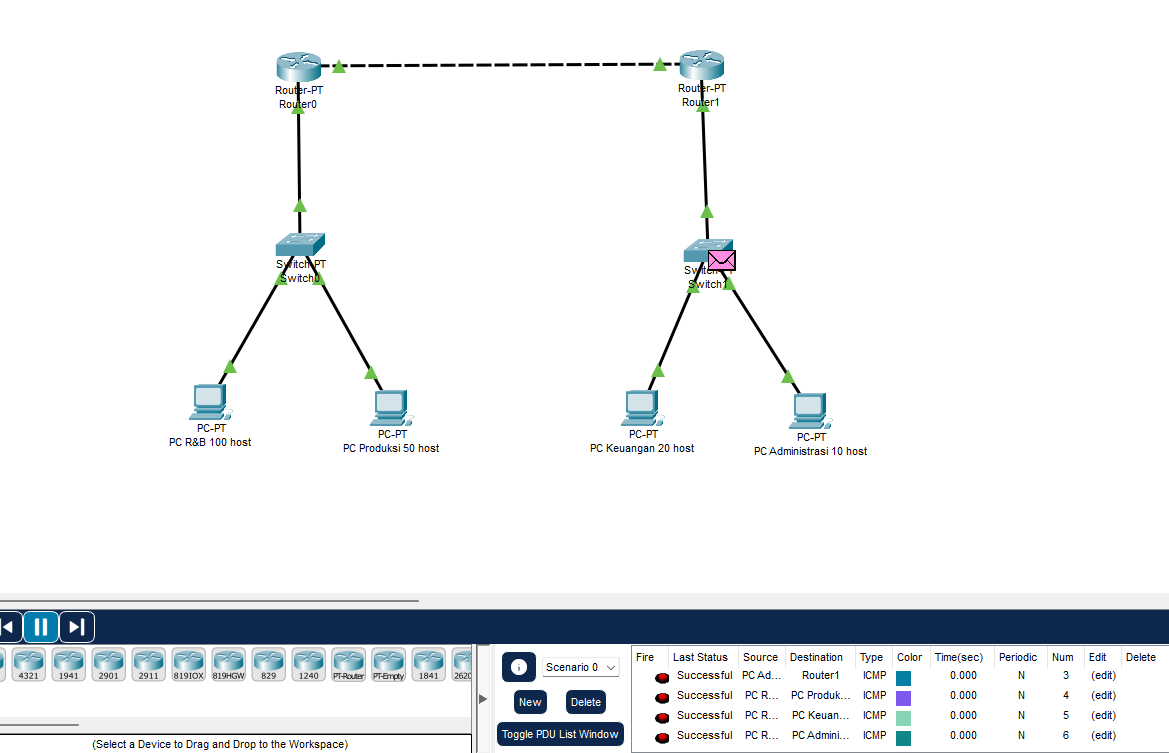
\includegraphics[width=0.8\textwidth]{P1/img/image.png}
        \caption{Simulasi Jaringan Menggunakan Cisco Packet Tracer}
        \label{fig:simulasi_jaringan}
    \end{figure}

    \item Jelaskan apa kesulitan yang anda alami pada Praktikum.
    \begin{itemize}
        \item kurang teliti saat melakukan crimping kabel LAN, sehingga ada beberapa kabel yang tidak terhubung dengan baik.
        \item kurang memahami langkah-langkah konfigurasi routing, sehingga mengalami kesulitan saat melakukan routing statis dan dinamis.
    \end{itemize}
\end{enumerate}


\section{Kesimpulan}
Berdasarkan hasil praktikum jaringan komputer, dapat disimpulkan bahwa praktikan berhasil melakukan crimping kabel LAN dengan standar T568B dan pengujian menggunakan LAN tester menunjukkan semua pin terhubung dengan baik, sesuai dengan teori. Praktikan juga berhasil melakukan konfigurasi routing statis antar dua jaringan, yang dibuktikan dengan koneksi berhasil melalui perintah ping. Namun, routing dinamis tidak dapat dilakukan karena keterbatasan waktu, lamanya pelaksanaan percobaan pertama, serta kurangnya pemahaman terhadap langkah-langkah konfigurasi routing dinamis. Secara keseluruhan, praktikum ini memberikan pemahaman praktis mengenai pembuatan kabel jaringan dan konfigurasi dasar routing, serta menjadi bahan evaluasi untuk meningkatkan persiapan dan efisiensi waktu pada praktikum selanjutnya.

\section{Lampiran}
\subsection{Dokumentasi saat praktikum}
\begin{figure}
    \centering
    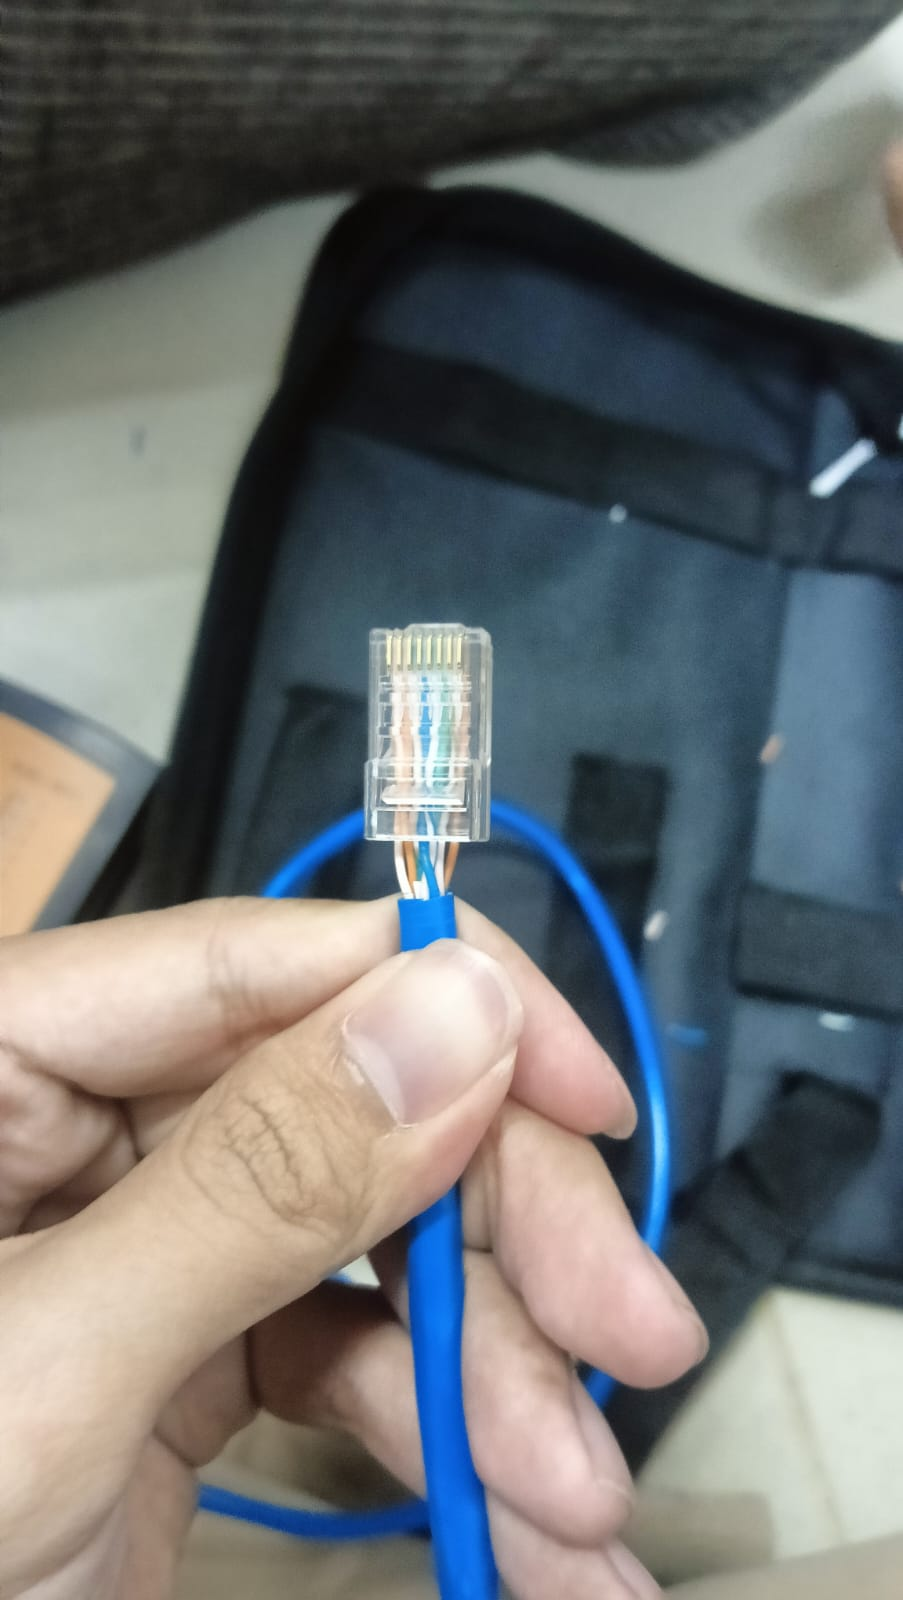
\includegraphics[width=0.8\textwidth]{P1/img/jk1 (1).jpg}
    \caption{Dokumentasi saat praktikum}
    \label{fig:dokumentasi_praktikum}
\end{figure}
\begin{figure}
    \centering
    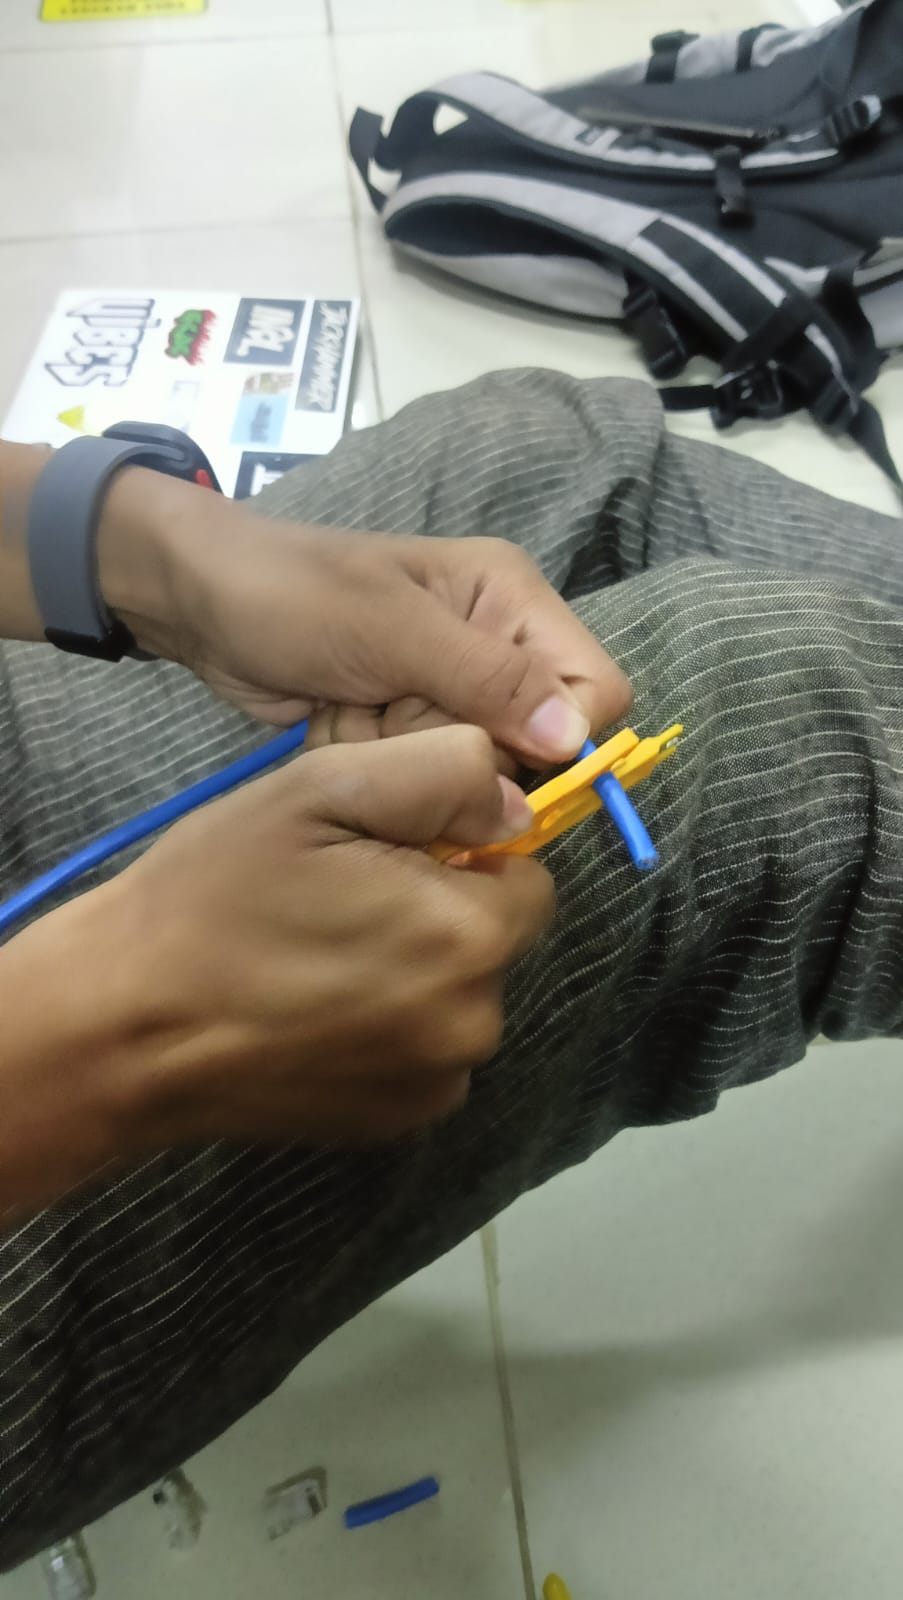
\includegraphics[width=0.8\textwidth]{P1/img/jk1 (2).jpg}
    \caption{Dokumentasi saat praktikum}
    \label{fig:dokumentasi_praktikum_2}
\end{figure}
\begin{figure}
    \centering
    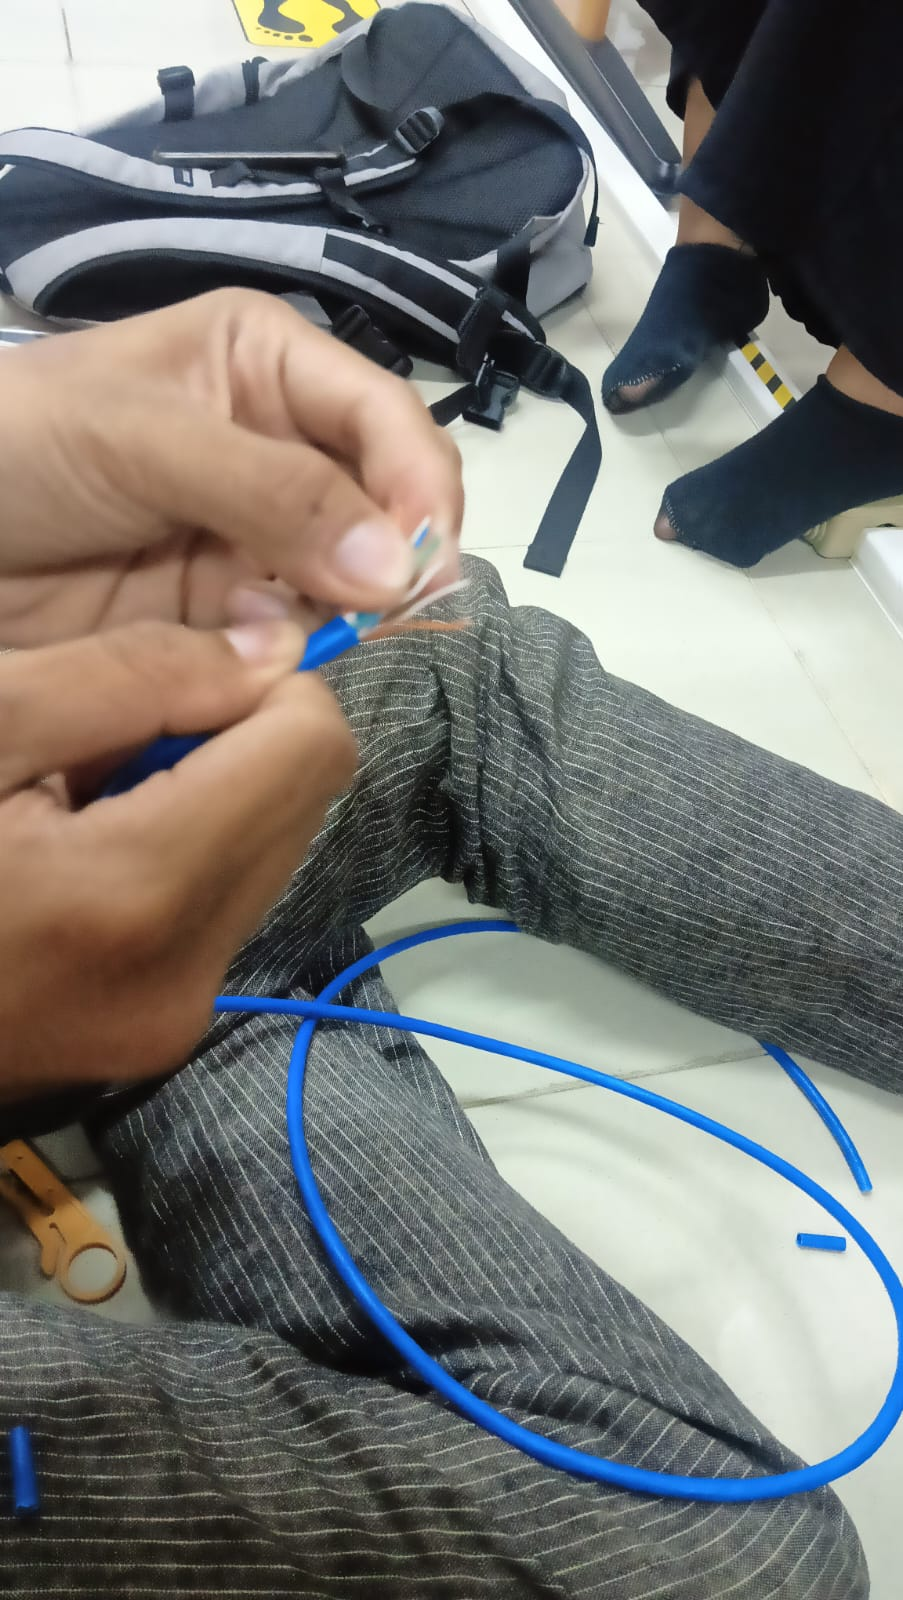
\includegraphics[width=0.8\textwidth]{P1/img/jk1 (3).jpg}
    \caption{Dokumentasi saat praktikum}
    \label{fig:dokumentasi_praktikum_3}
\end{figure}

\begin{figure}
    \centering
    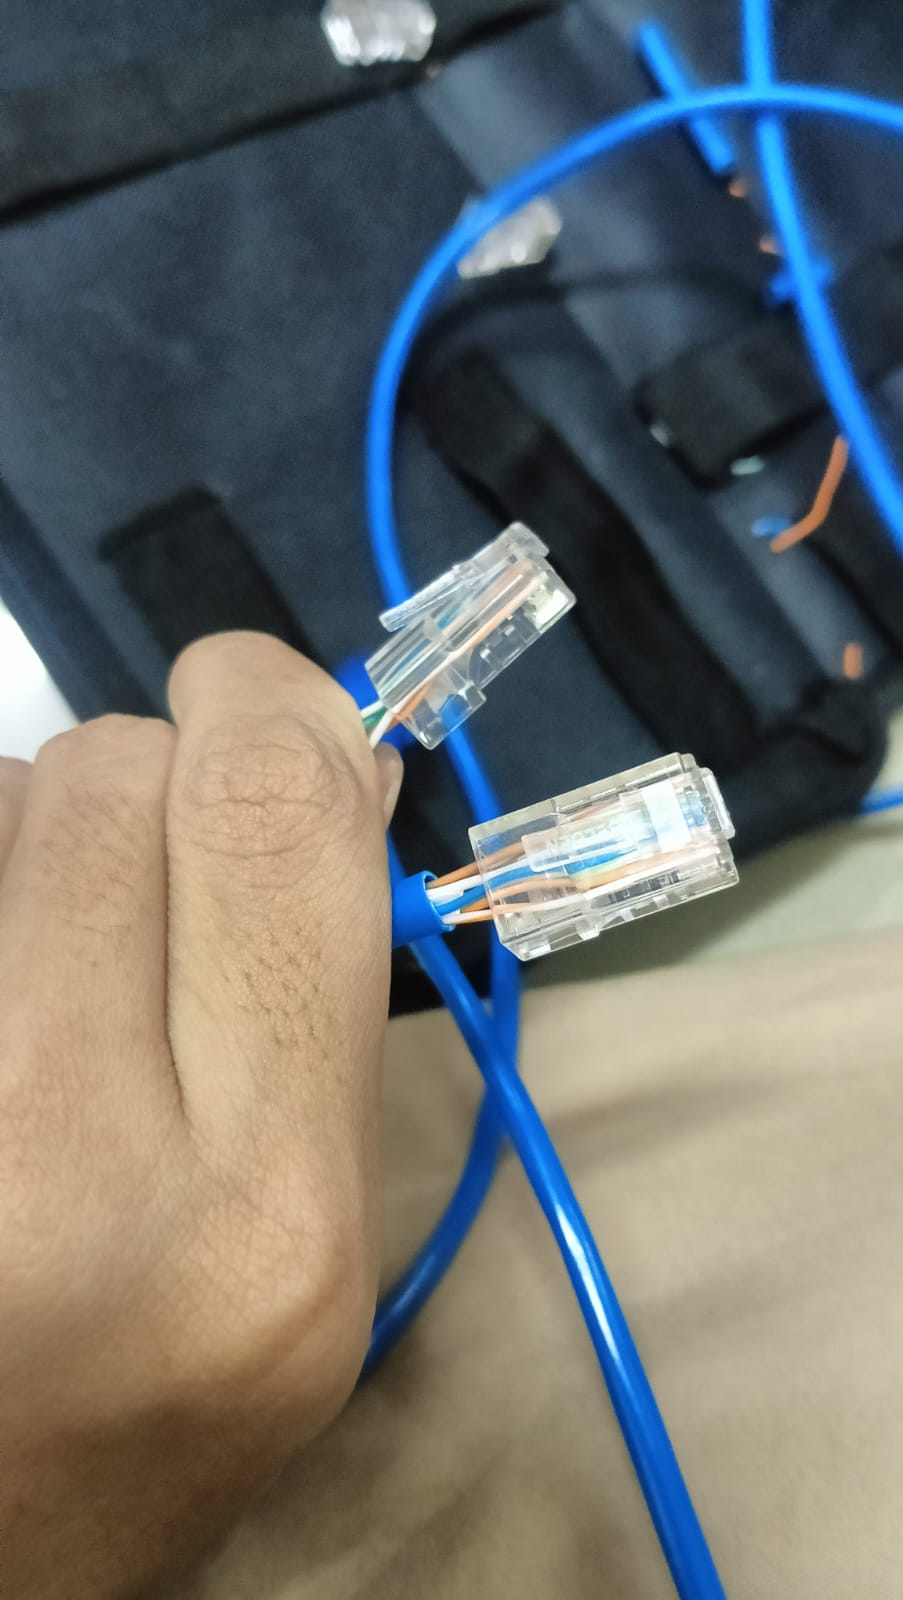
\includegraphics[width=0.8\textwidth]{P1/img/jk1 (5).jpg}
    \caption{Dokumentasi saat praktikum}
    \label{fig:dokumentasi_praktikum_5}
\end{figure}
\begin{figure}
    \centering
    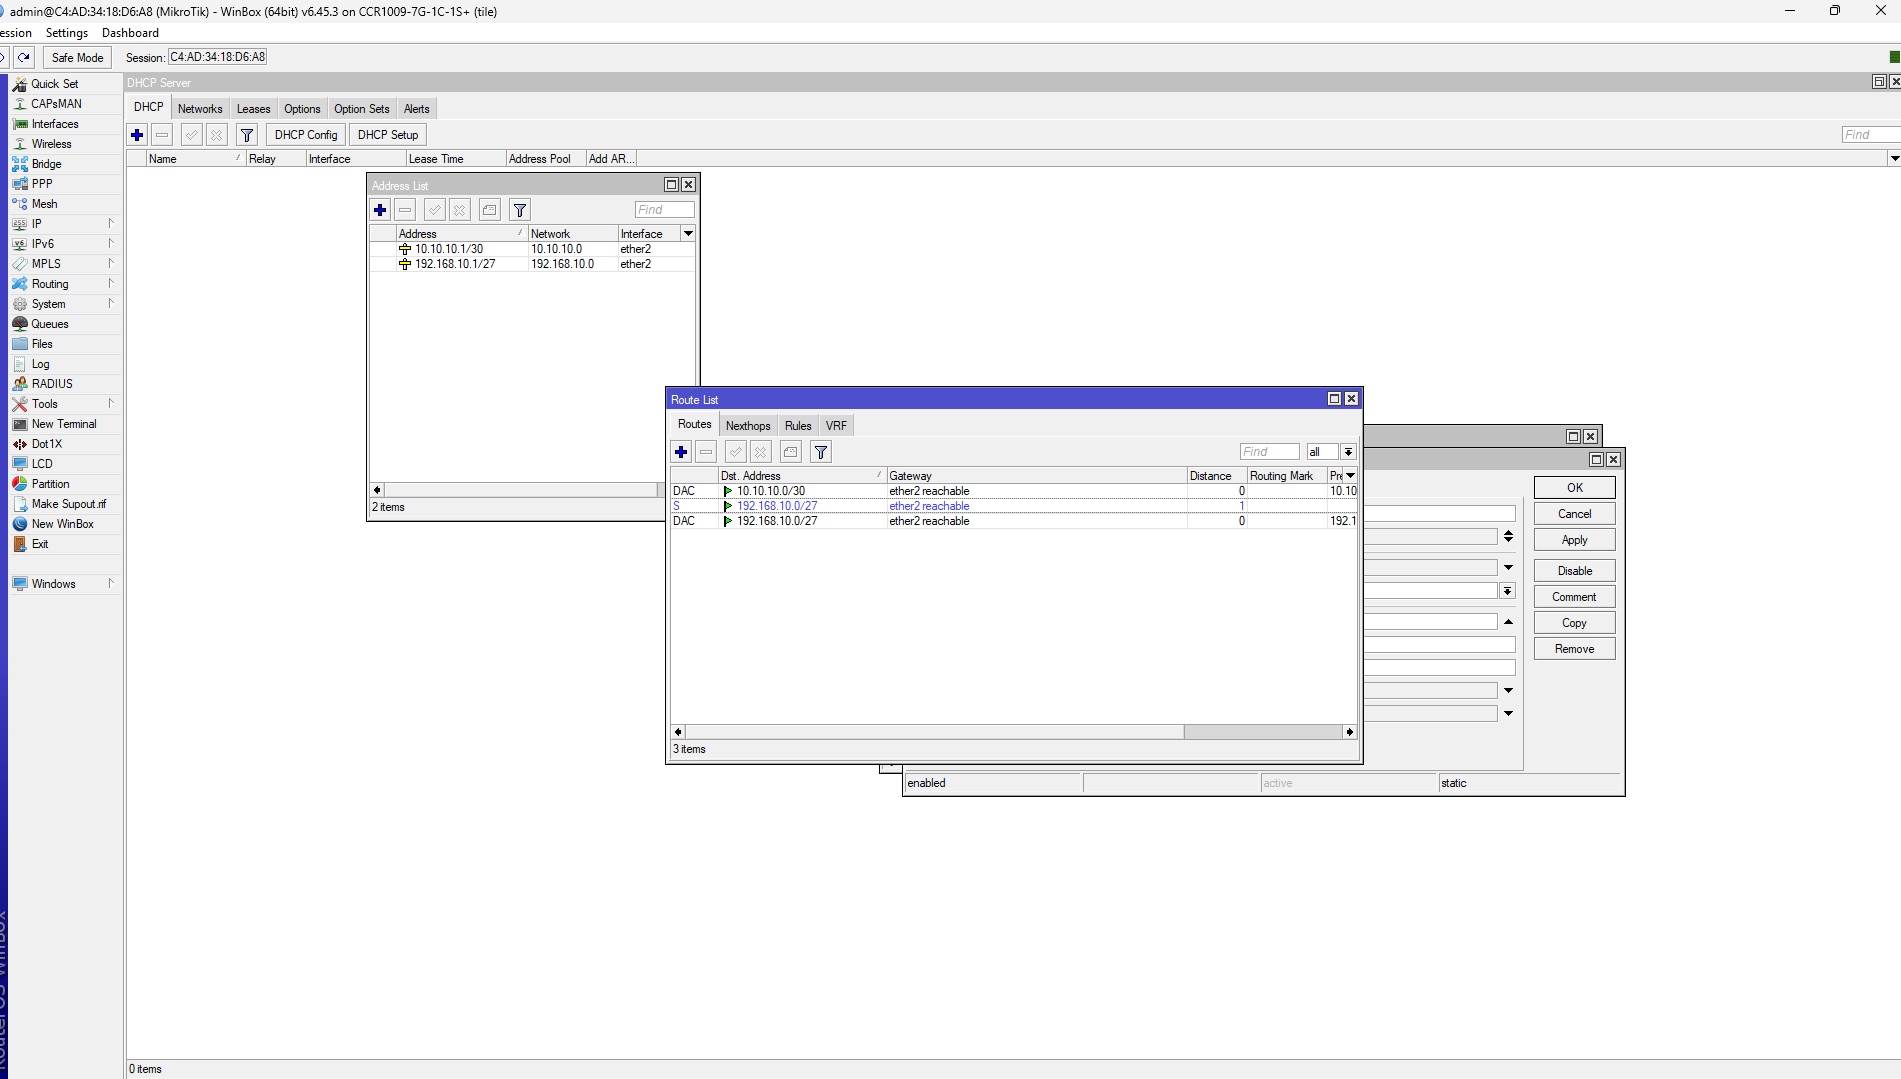
\includegraphics[width=0.8\textwidth]{P1/img/routing.png}
    \caption{Dokumentasi saat praktikum}
    \label{fig:dokumentasi_praktikum_6}
\end{figure}
\begin{figure}
    \centering
    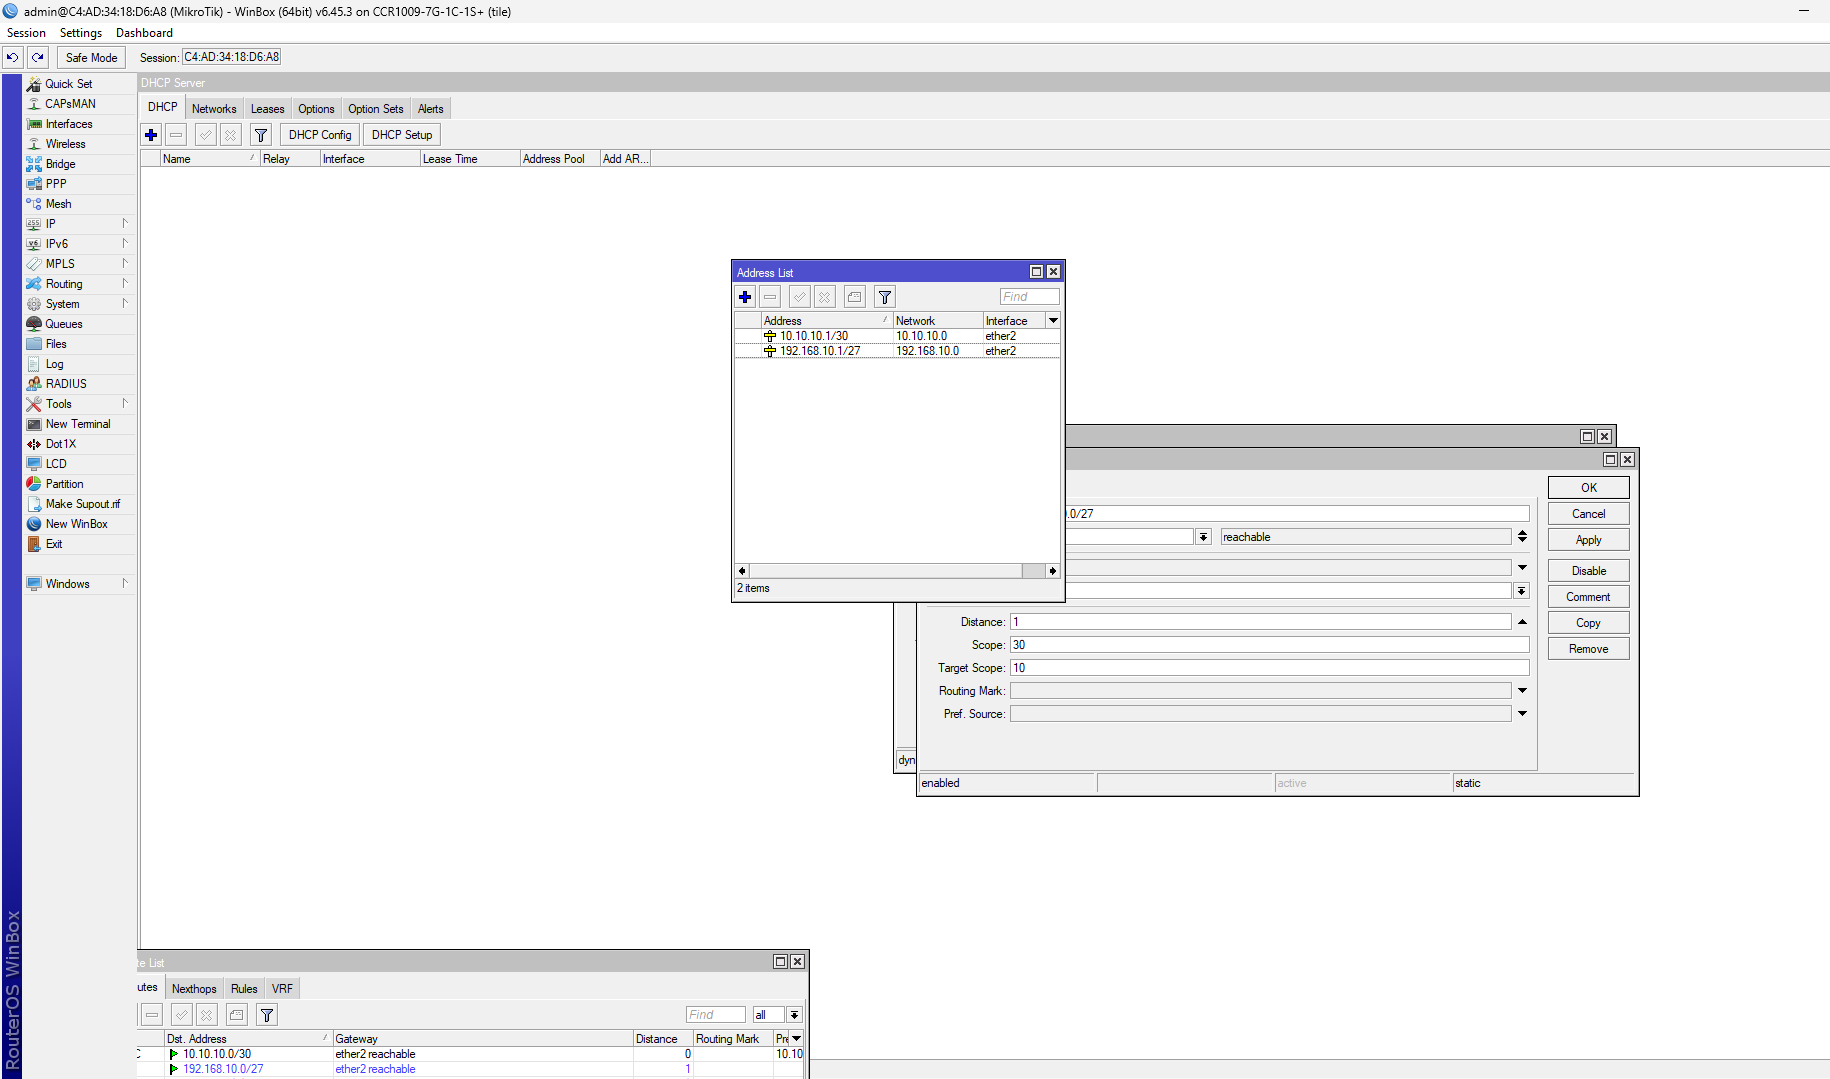
\includegraphics[width=0.8\textwidth]{P1/img/routing2.png}
    \caption{Dokumentasi saat praktikum}
    \label{fig:dokumentasi_praktikum_7}
\end{figure}
\begin{figure}
    \centering
    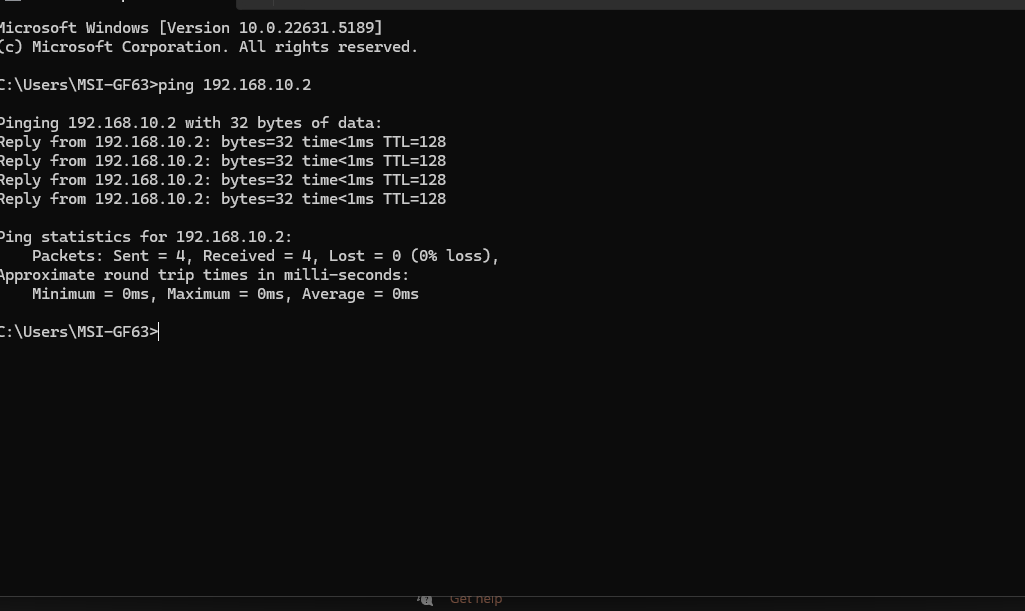
\includegraphics[width=0.8\textwidth]{P1/img/routing3.png}
    \caption{Dokumentasi saat praktikum}
    \label{fig:dokumentasi_praktikum_8}
\end{figure}